\documentclass[10pt]{amsart}
\usepackage{amsfonts}
\usepackage{amsmath}
\usepackage{amsthm}
\usepackage{amscd}

\usepackage[margin=1in]{geometry}
\usepackage[draft]{todonotes}

\usepackage{csquotes}
\usepackage{enumitem}
\usepackage{multicol}
\usepackage{caption}
\usepackage{tikz}
\usepackage{pgfplots}
\usepackage{minted}
\usepackage{nameref}
\usepackage{algpseudocode}
\usepackage{algorithm}
\usepackage{graphics}

\title{1D Finite Element Methods}
\author{Arden Rasmussen}
\date{\today}

\numberwithin{equation}{section}
\definecolor{red}{RGB}{244,67,54}
\definecolor{pink}{RGB}{233,30,99}
\definecolor{purple}{RGB}{156,39,176}
\definecolor{deep-purple}{RGB}{103,58,183}
\definecolor{indigo}{RGB}{117,125,232}
\definecolor{blue}{RGB}{110,198,255}
\definecolor{pale-blue}{RGB}{103,218,255}
\definecolor{cyan}{RGB}{98,239,255}
\definecolor{teal}{RGB}{82,199,184}
\definecolor{green}{RGB}{128,226,126}
\definecolor{pale-green}{RGB}{190,246,122}
\definecolor{lime}{RGB}{255,255,110}
\definecolor{yellow}{RGB}{255,255,114}
\definecolor{amber}{RGB}{255,243,80}
\definecolor{orange}{RGB}{255,201,71}
\definecolor{deep-orange}{RGB}{255,138,80}
\definecolor{brown}{RGB}{169,130,116}

\newenvironment{Figure}
{\par\medskip\noindent\minipage{\linewidth}}
{\endminipage\par\medskip}

\theoremstyle{definition}
\newtheorem{example}{Example}[section]

\newcommand{\pder}[2][]{\frac{\partial#1}{\partial#2}}
\newcommand{\spder}[2][]{\frac{\partial^2 #1}{\partial#2^2}}

\newcommand{\N}{\mathbb{N}}
\newcommand{\R}{\mathbb{R}}

\begin{document}
\maketitle
\begin{abstract}
  Finite Element Methods (FEM) is a process that is utilized to numerically
  approximate solutions to other wise impossible partial differential equations.
  This paper will serve as an explanation and introduction to the concept of
  FEM localized in one dimension.
\end{abstract}

\begin{multicols}{2}

  \section{Introduction}%
  \label{sec:introduction}

  We follow the process presented by \cite{KH}, for the Galerkin method for
  generating a finite element approximation in one dimension.

  For simplicity we will only examine FEM in one dimension. There ten stages for
  the implementation of the finite element analysis. The first four of which are
  theoretical, and must be done prior to numerical computation. These theoretical
  stages is used to setup the general mathematical formulas for computation, and
  is significantly more difficult to automate, and thus must be done
  analytically. The ten stages are listed below.

  \begin{enumerate}[label=(\roman*)]
    \item Problem Statement
    \item Variational Formulation
    \item Discretization
    \item Localization
    \item Mesh Generation
    \item Assembly of the Global System
    \item Incorporating Boundary Conditions
    \item Numerically Solving Algebraic System
    \item Repeating appropriate steps for time-dependent problems.
    \item Post processing.
  \end{enumerate}

  Due to the close dependence on the specific partial differential equation
  considered with the theoretical stages of the process, the results from these
  stages is closely dependent on the problem at hand. Because of this, we will use
  the steady 1D heat transfer model as our problem statement for this
  explanation.

  \section{Problem Statement}%
  \label{sec:problem_statement}

  We consider the steady 1D heat equation, which is a simplification of the
  unsteady multidimensional heat transfer model. Since the time derivative is
  neglected, there is no need for an initial condition, only a boundary condition
  for $T$ or $\pder[T]{x}$ at the endpoints of our considered interval is
  necessary

  \begin{equation}\label{eq:1d_heat_eq}
    \rho c_p u \pder[T]{x}-\pder{x}\left(k\pder[T]{x}\right)=f(x).
  \end{equation}

  Where $\rho$, $c_p$, $u$, and $k$ are constant. We take $f(x)$ to be the
  forcing function for the heat equation. We consider this on the domain
  $\Omega=(0,c)$. And we will prescribe the Dirichlet boundary conditions

  \begin{align*}
    T(0) = T_0\\
    T(c) = T_c.
  \end{align*}

  \section{Variational Formulation}%
  \label{sec:variational_formulation}

  We will define the residual of equation \eqref{eq:1d_heat_eq} as

  \begin{equation*}
    R(x) = \rho c_p u\pder[T]{x}-k\spder[T]{x}-f.
  \end{equation*}

  Clearly this equals $0$ if and only if $T$ is the exact solution. We then
  multiply the residual by some test function $w$ obtaining what is called the
  weighted residual

  \begin{equation*}
    \int_0^cw(x)R(x)dx=0.
  \end{equation*}

  For the exact solution, this will always be zero because $R(x)=0$. Thus we
  can select any function for our test function $w(x)$ and this will be true.

  This can be rewritten using integration by parts to obtain

  \begin{equation*}
    \rho c_p u\int_0^cw\pder[T]{x}dx+k\int_0^c\pder[w]{x}\pder[T]{x}dx-kw\pder[T]{x}\Bigr|_0^c=\int_0^cwfdx.
  \end{equation*}

  We now revise our problem to be finding a function $T$ that satisfies this
  expression. Because we apply our boundary conditions to the test function $w$
  we know that the test function is zero in the neighborhood of the boundaries
  by our definition of the test function $w(0)=w(c)=0$. Applying this fact
  provides the equation

  \begin{equation}\label{eq:cvp}
    \rho c_p
    u\int_0^cw\pder[T]{x}dx+k\int_0^c\pder[w]{x}\pder[T]{x}dx=\int_0^cwfdx.
  \end{equation}

  \section{Discretization}%
  \label{sec:discretization}

  Since the Sobolev spaces that the solution is contained in is infinitely
  dimensional, we will take the finite dimensional subspace $V_h\subset
  H^1((0,c))$ to create our approximation in. The Sobolev space $H^1((0,c))$ is
  the space of continuous functions that are infinitely differentiable. We will
  take a set of basis function $\left\{\varphi_j\right\}$. We leave these basis
  functions as arbitrary functions for now, and will show the process for
  selecting our basis functions.  We can then write our approximation $T_h$ of
  $T$ as a linear combination of this finite subspace

  \begin{equation}\label{eq:th}
    T_h=\sum_{j=1}^{N}T_j\varphi_j(x).
  \end{equation}

  Where $T_j$ are constants that we will solve for in a later stage.
  Substituting this into \eqref{eq:cvp} and taking our test function in this
  subspace $w_h=\varphi_i$, we find

  \begin{align*}
    \sum_{j=1}^{N}&\left[\rho c_pu
    \int_0^c\varphi_i\pder[\varphi_j]{x}dx\right]T_j\\
    &+
  \sum_{j=1}^{N}\left[k\int_0^c\pder[\varphi_i]{x}\pder[\varphi_j]{x}dx\right]T_j
    =\int_0^c\varphi_ifdx.
  \end{align*}

  We can write this system of equations for $i=1,\ldots,N$ as

  \begin{equation}\label{eq:matrix}
    (C+K)T=F.
  \end{equation}

  Where $T$ is vector in $\R^N$ of $T_j$ constants, and the elements of the
  matrices $C,K,F$ are given defined as

  \begin{align*}
    c_{ij}&=\rho c_p u\int_0^c\varphi_i\pder[\varphi_j]{x}dx\quad &i,j&=1,\ldots,N\\
    k_{ij}&=k\int_0^c\pder[\varphi_i]{x}\pder[\varphi_j]{x}dx\quad &i,j&=1,\ldots,N\\
    F_i&=\int_0^c\varphi_ifdx &i&=1,\ldots,N.
  \end{align*}

  Note that it is simpler to consider the matrix $A=C+K$ and use $A$ instead.

  \section{Localization}%
  \label{sec:localization}

  It is possible to find these matrices on the global domain, but that proves to
  be extremely difficult in higher dimensions, so we will use a generalizable
  method for the generation of these matrices. Since we are able to select our
  basis functions $\varphi_j$ we can carefully construct a set of basis
  functions such that it is possible to split the domain into elements. Where
  our element is a subset of the domain. We then determine the matrices for
  every element. Then using an algorithm we combine the element matrices to
  construct the global matrices.

  We discretize the domain using $N$ grid points $x_1<x_2<\cdots<x_N$ such that
  $x_1=0$ and $x_N=c$. Note that $N$ is the dimension of our basis functions
  $\left\{\varphi_j\right\}$ that were selected in section \ref{sec:discretization}. This will allow us to construct a mesh of $N-1$ elements
  defined as

  \begin{align*}
    E_e=\left[x_e,x_{e+1}\right]\quad\quad e=1,\ldots,N-1.
  \end{align*}

  For simplicity we will assume that all elements have the same size $h$,
  although different sizes can be easily handled.

  In order to construct our approximate solution, we define the shape function.
  We want all of our element basis functions to be of this shape function,
  in order to simplify the computations for the system

  \begin{align*}
    T_h^{(e)}=T_h\Bigr|_{E_e}\quad\quad e=1,\ldots,N-1.
  \end{align*}

  We approximate this shape function as some first-order polynomial. Note that
  for higher accuracy it is possible to approximate the shape function as a
  higher order polynomial, but for simplicity we utilize first-order
  polynomials

  \begin{align}\label{eq:the}
    T_h^{(e)}(x)=\alpha_1^{(e)}+\alpha_2^{(e)}x\quad\quad
    x\in\left[x_e,x_{e+1}\right].
  \end{align}

  Then because we want $T_h$ to be continuous, we must apply the boundaries
  of the element to the shape function

  \begin{align*}
  &T_h^{(e)}(x_e)=T_1^{(e)}\equiv T_h(x_e)\\
  &T_h^{(e)}(x_{e+1})=T_2^{(e)}\equiv T_h(x_{e+1}).
  \end{align*}

  Evaluating this expression and solving for $\alpha_1^{(e)}$ and
  $\alpha_2^{(e)}$ results in

  \begin{align*}
    \alpha_1^{(e)}&=eT_1^{(e)}-(e-1)T_2^{(e)}\\
    \alpha_2^{(e)}&=\frac{1}{h}\left(T_2^{(e)}-T_1^{(e)}\right).
  \end{align*}

  Using these results we substitute them into \eqref{eq:the}, and find

  \begin{align*}
    T_h^{(e)}&=eT_1^{(e)}-(e-1)T_2^{(e)}+\frac{1}{h}\left(T_2^{(e)}-T_1^{(e)}\right)x\\
             &=T_1^{(e)}\left(\frac{-x}{h}+e\right)+T_2^{(e)}\left(\frac{x}{h}-e+1\right)\\
             &=T_1^{(e)}\varphi_1^{(e)}(x)+T_2^{(e)}\varphi_2^{(e)}(x).
  \end{align*}

  Thus we define our local basis functions $\varphi_1^{(e)}$ and
  $\varphi_2^{(e)}$ as

  \begin{align}\label{eq:local_basis}
    \varphi_1^{(e)}&=\frac{-x}{h}+e\\
    \varphi_2^{(e)}&=\frac{x}{h}-e+1.
  \end{align}

  Thus for every element there is a pair of local basis functions, and a local
  shape function. A plot of these local basis functions is shown in
  figure \ref{fig:local_basis}.

  \begin{Figure}
    \begin{center}
      \begin{tikzpicture}[scale=4]
        \draw (-0.2,0) -- (0,0) node[below]{$e$} -- node[above]{$E_e$} (1,0) node[below]{$e+1$} -- (1.2,0);
        \draw (0,1) node[above]{$\varphi_1^{(e)}$} -- (1,0);
        \draw (0,0) -- (1,1) node[above]{$\varphi_2^{(e)}$};
        \draw[dotted] (0,0) -- node[left]{$1$} (0,1);
        \draw[dotted] (1,0) -- node[right]{$1$} (1,1);
        % \draw[very thin,color=gray] (-0.1,-1.1) grid (3.9,3.9);
      \end{tikzpicture}
    \end{center}
    \captionof{figure}{Local basis functions $\varphi_1^{(e)}$ and
    $\varphi_2^{(e)}$ on element $e$.}
    \label{fig:local_basis}
  \end{Figure}

  The global approximation is then found as a linear combination
  of global basis functions, which we now define as a piecewise combination of
  local basis functions. We construct our global basis functions $\varphi_j(x)$
  as the combination of local basis functions such that at grid point $j$ it is
  equal to $1$ and at all other grid points is zero, as seen in figure
  \ref{fig:global_basis}.

  \begin{Figure}
    \begin{center}
      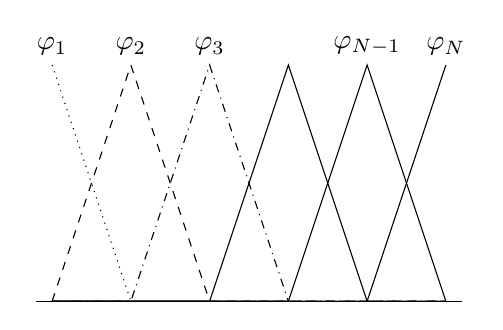
\begin{tikzpicture}[scale=1, transform shape]
        \draw (-0.2,0)--(0,0)--(5,0)--(5.2,0);
        \draw[dotted] (0,3) node[above]{$\varphi_1$}--(1,0)--(2,0)--(3,0)--(5,0);
        \draw[dashed] (0,0)--(1,3) node[above]{$\varphi_2$}--(2,0)--(3,0)--(5,0);
        \draw[dashdotted] (0,0)--(1,0)--(2,3) node[above]{$\varphi_3$}--(3,0)--(5,0);
        \draw (0,0)--(1,0)--(2,0)--(3,3)--(4,0)--(5,0);
        \draw (0,0)--(1,0)--(2,0)--(3,0)--(4,3) node[above]{$\varphi_{N-1}$}--(5,0);
        \draw (0,0)--(1,0)--(2,0)--(3,0)--(4,0)--(5,3)node[above]{$\varphi_N$};
    \end{tikzpicture}
  \end{center}
  \captionof{figure}{Global basis functions $\varphi_j(x)$.}
  \label{fig:global_basis}
\end{Figure}

Because of this construction of the global basis functions, we are able to
represent them in terms of our local basis functions

\begin{align*}
  \varphi_1(x)&=\begin{cases}
    \varphi_1^{(1)}(x) & x\in E_1=(0,h)\\
    0 & elsewhere
  \end{cases}\\
  \varphi_2(x)&=\begin{cases}
    \varphi_2^{(1)}(x) & x\in E_1=(0,h)\\
    \varphi_1^{(2)}(x) & x\in E_2=(h,2h)\\
    0 & elsewhere
  \end{cases}\\
              & \vdots \\
  \varphi_N(x)&=\begin{cases}
    \varphi_2^{(N-1)}(x) & x\in E_{N-1}\\
    0 & elsewhere
  \end{cases}.
\end{align*}

Thus from this construction we find that our general expression for the global
basis function which is not on a boundary such as $j=0$ and $j=N$ is as follows

\begin{align}
  \varphi_j(x)=\begin{cases}
    \frac{x}{h}-j+2 & x \in ((j-2)h,(j-1)h)\\
    \frac{-x}{h}+j & x \in ((j-1)h,jh)\\
    0 & elsewhere
  \end{cases}.
\end{align}

We are now able to use this definition of our basis function to apply in the
construction of an element specific system of equations from \eqref{eq:matrix}.

Thus we construct our local system of equations in matrix form as

\begin{align}
  \left(C^{(e)}+K^{(e)}\right)T^{(e)}=F^{(e)}.
\end{align}

Here the elements of each matrix is determined by our local basis functions, and
the size of the matrix is equivalent to the number of local degrees of freedom,
which in this case is two (One for each end point of an element). The elements
of these matrices are found through the following

\begin{align*}
  c_{ij}^{(e)}&=\rho c_p u\int_{E_e}\varphi_i^{(e)}\pder[\varphi_j^{(e)}]{x}dx\quad
              &i,j&=1,2\\
  k_{ij}^{(e)}&=k\int_{E_e}\pder[\varphi_i^{(e)}]{x}\pder[\varphi_j^{(e)}]{x}dx\quad
              &i,j&=1,2\\
  F_i^{(e)}&=\int_{E_e}\varphi_i^{(e)}fdx &i&=1,2.
\end{align*}

\section{Mesh Generation}%
\label{sec:mesh_generation}

To generate a mesh in 1D is to simply split the domain of our problem into a
set of finite elements. We select the number of grid points that are desired
$N$. Then the number of elements that will be produced is $N-1$. For the 1D
problem we will simply divide the domain $\Omega=(0,c)$ into $N-1$ evenly sized
elements. Thus each interval with have length $h=\frac{c}{N-1}$. Note that the
greater the number of elements will results in a higher accuracy approximation,
but will be at the cost of computational complexity.

\section{Assembly of the Global System}%
\label{sec:assembly_of_the_global_system}

It is possible to directly construct the global matrix based, however this
method is ineffective for practical computation and so in this introduction will
be ignored.

The method that will be used is an incremental construction of the global
matrix, by the addition of elements from the local matrices. We begin by
initializing the matrix $A=C+K$ and $F$ of zeros, in one dimension both of these
matrices are $N\times N$. Then the corresponding contributions of the element
matrices $A^{(e)}=C^{(e)}+K^{(e)}$ and $F^{(e)}$ are added in a loop over all
elements.

\begin{algorithm}[H]
  \caption{element-by-element assembly}
  \begin{algorithmic}
    \State{Let $A$ be a $N\times N$ matrix of zeros.}
    \State{Let $F$ be a $N\times 1$ matrix of zeros.}
    \ForAll{$E_e$}
    \State{Let $A^{(e)}$ be a $2\times 2$ matrix, such that}
    \State{$A_{IJ}^{(e)}=c_{IJ}^{(e)}+k_{IJ}^{(e)},\quad I,J=1,2$}
    \State{Determine relation between global and local node numbers.}
    \State{$i=node(e,I)\quad j=node(e,J)\quad I,J=1,2$}
    \State{Update the global $A$ matrix.}
    \State{$A_{ij}=A_{ij}+A_{IJ}^{(e)}\quad I,J=1,2$}
    \State{Update the global $F$ matrix.}
    \State{$F_i=F_i+F_I^{(e)}\quad I=1,2$}
    \State{In our construction of the element mesh the relation between
    global and local is given like so}
    \State{$node(e,1)=e\quad node(e,2)=e+1$}
    \EndFor
    \State{\Return{$A$, and $F$.}}
  \end{algorithmic}
\end{algorithm}

We demonstrate the results of this algorithm with an example.

\begin{example}
  We will construct a global matrix for the element mesh with three elements.
  Thus $N=4$.

  We take $A^{(e)}$ to be a $2\times 2$ matrix with elements defined as

  \begin{align*}
    A_{ij}^{(e)}=\rho c_p u \int_{E_e}\varphi_i^{(e)}\pder[\varphi_j^{(e)}]{x}dx+
    k\int_{E_e}\pder[\varphi_i^{(e)}]{x}\pder[\varphi_j^{(e)}]{x}dx.
  \end{align*}

  And $F^{(e)}$ is a $2\times 1$ matrix with elements defined as

  \begin{align*}
    F_i^{(e)}=\int_{E_e}\varphi_i^{(e)}fdx.
  \end{align*}

  Using these two matrices, we construct the global matrix for $N=4$ to be

  \begin{align*}
    A&=\begin{pmatrix}
      A_{11}^{(1)} & A_{12}^{(1)} & 0 & 0\\
      A_{21}^{(1)} & A_{22}^{(1)}+A_{11}^{(2)} & A_{12}^{(2)} & 0\\
      0 & A_{21}^{(2)} & A_{22}^{(2)}+A_{11}^{(3)} & A_{12}^{(3)}\\
      0 & 0 & A_{21}^{(3)} & A_{22}^{(3)}
    \end{pmatrix}\\
    F&=\begin{pmatrix}
      F_1^{(1)}\\
      F_2^{(1)}+F_1^{(2)}\\
      F_2^{(2)}+F_1^{(3)}\\
      F_2^{(3)}
    \end{pmatrix}.
  \end{align*}
\end{example}

Using this algorithm, it is simple to construct the global $A$, and $F$
matrices. It also becomes clear that the matrix of $A$ is a tridiagonal
matrix (At least in this one dimensional case).

\section{Dirichlet Boundary Conditions}%
\label{sec:section_name}

With our global system of equations constructed in the general form of

\begin{align}\label{eq:global_sys}
  \begin{pmatrix}
    a_{11} & a_{12} & \cdots & a_{1N}\\
    a_{21} & a_{22} & \cdots & a_{2N}\\
    \vdots & \vdots & \ddots & \vdots \\
    a_{N1} & a_{N2} & \cdots & a_{NN}
  \end{pmatrix}
  \begin{pmatrix}
    T_1 \\ T_2 \\ \vdots \\ T_N
  \end{pmatrix}
  =
  \begin{pmatrix}
    F_1 \\ F_2 \\ \vdots \\ F_N
  \end{pmatrix}.
\end{align}

This solution is not well behaved, as we have neglected the prescribed boundary
conditions until now. This means that our matrix is over determined and cannot
be solved, to fix this we must apply our boundary conditions. As we know from
our Dirichlet boundary conditions that

\begin{align*}
  T_1&=T_0\\
  T_N&=T_c.
\end{align*}

There are several ways of applying these boundary conditions to the system of
equations, but we will focus on a single method. This method is to leave the
boundary values of $T_i$ as if they were unknown, and simply modify the system
of equations such that they are forced to appear. This is done by modifying two
of the equations of the system. This modification can be done to any two
equations of the system, but in order to maintain the tridiagonality of this
matrix, we will modify the first and last equations in the system. This can be done like so

\begin{align*}
  \resizebox{\columnwidth}{!}{$
  \begin{pmatrix}
    1 & 0 & \cdots & 0\\
    a_{21} & a_{22} & \cdots & a_{2N}\\
    \vdots & \vdots & \ddots & \vdots \\
    a_{(N-1)1} & a_{(N-1)2} & \cdots & a_{(N-1)N}\\
    0 & 0 & \cdots & 1
  \end{pmatrix}
  \begin{pmatrix}
    T_1 \\ T_2 \\ \vdots \\ T_{N-1} \\ T_N
  \end{pmatrix}
  =
  \begin{pmatrix}
    T_0 \\ F_2 \\ \vdots \\ F_{N-1} \\ T_c
\end{pmatrix}.$}
\end{align*}

Using this system of equations is easy to implement, and allows for easy
solving as it retains the tridiagonal nature of the matrix $A$.

\section{Solving the Algebraic System}%
\label{sec:solving_the_algebraic_system}

In order to solve the system of equations we must find the values for all
$a_{ij}$ and the values for $F_{i}$. The process for finding each of these is
given, and since $f(x)$ is given as an input as the forcing function, we are
able to numerically solve for all of these values.

Due to the tridiagonal nature of the matrix, it allows the implementation of
extremely efficient algorithms to find the solution, that can obtain a solution
in $O(n)$ operations instead of the normal $O\left(n^3\right)$ required by
Gaussian elimination.

This algorithm is outlined below for a system of equations of the general form

\begin{align*}
  \begin{pmatrix}
    b_1 & c_1 & 0 & \cdots & 0 \\
    a_2 & b_2 & c_2 & \cdots & 0\\
    0 & a_3 & b_3 & \ddots & \vdots\\
    \vdots & \vdots & \ddots & \ddots & c_{n-1}\\
    0 & 0 & \cdots & a_n & b_n
  \end{pmatrix}
  \begin{pmatrix}
    x_1 \\ x_2 \\ x_3 \\ \vdots \\ x_n
  \end{pmatrix}
  =
  \begin{pmatrix}
    d_1 \\ d_2 \\ d_3 \\ \vdots \\ d_n
  \end{pmatrix}.
\end{align*}

\begin{algorithm}[H]
  \caption{Thomas algorithm}
  \begin{algorithmic}
    \For{$i \in 1,2,\ldots,n-1$}
    \If{$i=1$}
    \State{$c_i=\frac{c_i}{b_i}$}
    \State{$d_i=\frac{d_i}{b_i}$}
    \ElsIf{$i\neq n$}
    \State{$c_i=\frac{c_i}{b_i-a_ic_{i-1}}$}
    \State{$d_i=\frac{d_i-a_id_{i-1}}{b_i-a_ic_{i-1}}$}
    \ElsIf{$i=n$}
    \State{$d_i=\frac{d_i-a_id_{i-1}}{b_i-a_ic_{i-1}}$}
    \EndIf
    \EndFor
    \For{$i \in n,\ldots,1$}
    \If{$i=n$}
    \State{$x_i=d_i$}
    \Else
    \State{$x_i=d_i-c_ix_{i+1}$}
    \EndIf
    \EndFor
    \State{\Return $X$}
  \end{algorithmic}
\end{algorithm}

This algorithm will efficiently determine the solution to our system of
equations.  A note about tridiagonal matrices is they are extremely efficient
computationally. As only the three diagonals are needed to be stored as all
other elements are zero. Because of this the memory for an $N\times N$ matrix
can be reduced to the memory needed for a $N\times 3$ matrix. Which for very
large number of elements will be extremely substantial.

This along with the efficiency of computing solutions to tridiagonal systems of
equations indicates that maintaining the tridiagonality of the matrix is very
useful.

We can then construct our final approximation of $T$ like so

\begin{align}
  T_h(x) = T_0\varphi_1(x)+T_c\varphi_N(x)+\sum_{j=2}^{N-1}T_j\varphi_j(x).
\end{align}


\section{Further Iterations}%
\label{sec:further_iterations}

Because of our choice of differential equation, and our decision to neglect the
time derivative, indicates that $T_h(x)$ is our final solution.

\section{Postprocessing}%
\label{sec:postprocessing}

This stage is to display the approximation of the solution, and to generate
graphs or calculate errors. This step is entirely dependent on the example at
hand and the desired use of FEA. Due to this we will skip this step for now.

\section{Example Problem}%
\label{sec:example_problem}

For additional clarity we will implement this process on an example problem to
demonstrate the stages, and the problem specific steps.

\subsection{Problem Statement}%
\label{sub:problem_statement}

We will continue to use the steady 1D heat equation

\begin{align*}
  \rho c_p y\pder[T]{x}-\pder{x}\left(k\pder[T]{x}\right)=f.
\end{align*}

We will use the domain $\Omega=(0,c)=(0,5)$.

We will define $f(x)$ to be

\begin{align*}
  f(x)=\frac{\xi\pi}{c}\left[\rho c_p
  u\cos\left(\frac{\xi\pi}{c}x\right)+k\frac{\xi\pi}{c}\sin\left(\frac{\xi\pi}{c}x\right)\right].
\end{align*}

Where $\xi \in \N$, in our example we will take $\xi=2$. And we will take
$N=4$. And finally we apply our Dirichlet boundary conditions to be

\begin{align*}
  T_1=T(0)=0\\
  T_2=T(5)=0.
\end{align*}

\subsection{Variational Formulation}%
\label{sub:variational_formulation}

As the variational formulation only depended on the differential equation,
which we have kept the same, this step is identical to as it was in the
explanation.

\subsection{Discretization}%
\label{sub:discretization}

Again, the discretization of the problem was only dependent on the differential
equation. Thus we can use the same expression for the global system $(C+K)T=F$
that were found in the explanation.

\subsection{Localization}%
\label{sub:localization}

The localization process is only dependent on the dimension of the problem. So
for any FEA contained in one dimension will utilize the same
$\varphi_i^{(e)}(x)$ and $\varphi_i(x)$. The only difference could come from
the construction of the local matrix $C^{(e)}$, $K^{(e)}$, and $F^{(e)}$. But
this process stems from the discretization process, and thus only depends on
the differential equation. Which in our case has remained the same.

\subsection{Mesh Generation}%
\label{sub:mesh_generation}

This is the first stage where some difference occurs, as it is the first
computational stage. We are able to generate the mesh of elements, which in the
one dimensional case is trivial. We take the set of node points

\begin{align*}
  x = \left\{0, \frac{5}{3}, \frac{10}{3}, 5\right\}.
\end{align*}

\subsection{Assembly of the Global System}%
\label{sub:assembly_of_the_global_system}

The process for assembling the global system is identical as in the
explanation. However, with our example problem we are able to numerically solve
for our global $A$ and $F$ matrices. These matrices become

\begin{align*}
  A&=\begin{pmatrix}
    0.1 & -0.1 & 0.0 & 0.0 \\
    -1.1 & 1.2 & -0.1 & 0.0 \\
    0.0 & -1.1 & 1.2 & -0.1 \\
    0.0  & 0.0 & -1.1 & 1.1
  \end{pmatrix}\\
  F&=\begin{pmatrix}
    1.453 \\ 0.842 \\ -2.275 \\ -0.021
  \end{pmatrix}.
\end{align*}

Thus our global system can be represented as

\begin{align*}
  \begin{pmatrix}
    0.1 & -0.1 & 0.0 & 0.0 \\
    -1.1 & 1.2 & -0.1 & 0.0 \\
    0.0 & -1.1 & 1.2 & -0.1 \\
    0.0  & 0.0 & -1.1 & 1.1
  \end{pmatrix}
  \begin{pmatrix}
    T_1 \\ T_2 \\ T_3 \\ T_4
  \end{pmatrix}
  =
  \begin{pmatrix}
    1.453 \\ 0.842 \\ -2.275 \\ -0.021
  \end{pmatrix}.
\end{align*}

\subsection{Dirichlet Boundary Conditions}%
\label{sub:dirichlet_boundary_conditions}

Once again we use the process to apply our Dirichlet boundary conditions to the
system of equations. Thus obtaining

\begin{align*}
  \begin{pmatrix}
    1.0 &  0.0 & 0.0 & 0.0 \\
    -1.1 & 1.2 & -0.1 & 0.0 \\
    0.0 & -1.1 & 1.2 & -0.1 \\
    0.0 &  0.0 & 0.0 & 1.0
  \end{pmatrix}
  \begin{pmatrix}
    T_1 \\ T_2 \\ T_3 \\ T_4
  \end{pmatrix}
  =
  \begin{pmatrix}
    0.000 \\ 0.842 \\ -2.275 \\ 0.000
  \end{pmatrix}.
\end{align*}

\subsection{Solving the Algebraic System}%
\label{sub:solving_the_algebraic_system}

Using our algorithm for solving tridiagonal matrices, we are able to find the
values for $T_i$ to be

\begin{align*}
  T=\begin{pmatrix}
    0.000000 \\ 0.589228 \\ -1.355743 \\ 0.000000
  \end{pmatrix}.
\end{align*}

Thus resulting in our final approximation to be

\begin{align*}
  T_h(x) = 0.589228\varphi_2(x)-1.355743\varphi_3(x).
\end{align*}

\subsection{Further Iterations}%
\label{sub:further_iterations}

Again as we neglect the time derivative $T_h(x)$ is our final solution.

\subsection{Postprocessing}%
\label{sub:postprocessing}

Now that we have an actual solution to our expression we are able to do some
post processing.

We claim that a solution to this differential equation can be found analytically
to be

\begin{align*}
  T(x) = \sin\left(\frac{\xi\pi}{c}x\right).
\end{align*}

Using the analytical solution, and our FEM approximation, we are able to plot
each solution and compare the error function between the actual and our
approximate solutions.

\begin{Figure}
   \begin{center}
     \begin{tikzpicture}
\definecolor{color0}{RGB}{0,0,0}
\definecolor{color1}{RGB}{0,0,0}
\begin{axis}[axis lines = middle, xmin=0.000000, xmax=4.975000, ymin=-1.446018,
ymax=1.400000]
\addplot[color0, dashed, forget plot]
table{%
0.000000 0.000000
0.025000 0.031411
0.050000 0.062791
0.075000 0.094108
0.100000 0.125333
0.125000 0.156434
0.150000 0.187381
0.175000 0.218143
0.200000 0.248690
0.225000 0.278991
0.250000 0.309017
0.275000 0.338738
0.300000 0.368125
0.325000 0.397148
0.350000 0.425779
0.375000 0.453990
0.400000 0.481754
0.425000 0.509041
0.450000 0.535827
0.475000 0.562083
0.500000 0.587785
0.525000 0.612907
0.550000 0.637424
0.575000 0.661312
0.600000 0.684547
0.625000 0.707107
0.650000 0.728969
0.675000 0.750111
0.700000 0.770513
0.725000 0.790155
0.750000 0.809017
0.775000 0.827081
0.800000 0.844328
0.825000 0.860742
0.850000 0.876307
0.875000 0.891007
0.900000 0.904827
0.925000 0.917755
0.950000 0.929776
0.975000 0.940881
1.000000 0.951057
1.025000 0.960294
1.050000 0.968583
1.075000 0.975917
1.100000 0.982287
1.125000 0.987688
1.150000 0.992115
1.175000 0.995562
1.200000 0.998027
1.225000 0.999507
1.250000 1.000000
1.275000 0.999507
1.300000 0.998027
1.325000 0.995562
1.350000 0.992115
1.375000 0.987688
1.400000 0.982287
1.425000 0.975917
1.450000 0.968583
1.475000 0.960294
1.500000 0.951057
1.525000 0.940881
1.550000 0.929776
1.575000 0.917755
1.600000 0.904827
1.625000 0.891007
1.650000 0.876307
1.675000 0.860742
1.700000 0.844328
1.725000 0.827081
1.750000 0.809017
1.775000 0.790155
1.800000 0.770513
1.825000 0.750111
1.850000 0.728969
1.875000 0.707107
1.900000 0.684547
1.925000 0.661312
1.950000 0.637424
1.975000 0.612907
2.000000 0.587785
2.025000 0.562083
2.050000 0.535827
2.075000 0.509041
2.100000 0.481754
2.125000 0.453990
2.150000 0.425779
2.175000 0.397148
2.200000 0.368125
2.225000 0.338738
2.250000 0.309017
2.275000 0.278991
2.300000 0.248690
2.325000 0.218143
2.350000 0.187381
2.375000 0.156434
2.400000 0.125333
2.425000 0.094108
2.450000 0.062791
2.475000 0.031411
2.500000 0.000000
2.525000 -0.031411
2.550000 -0.062791
2.575000 -0.094108
2.600000 -0.125333
2.625000 -0.156434
2.650000 -0.187381
2.675000 -0.218143
2.700000 -0.248690
2.725000 -0.278991
2.750000 -0.309017
2.775000 -0.338738
2.800000 -0.368125
2.825000 -0.397148
2.850000 -0.425779
2.875000 -0.453990
2.900000 -0.481754
2.925000 -0.509041
2.950000 -0.535827
2.975000 -0.562083
3.000000 -0.587785
3.025000 -0.612907
3.050000 -0.637424
3.075000 -0.661312
3.100000 -0.684547
3.125000 -0.707107
3.150000 -0.728969
3.175000 -0.750111
3.200000 -0.770513
3.225000 -0.790155
3.250000 -0.809017
3.275000 -0.827081
3.300000 -0.844328
3.325000 -0.860742
3.350000 -0.876307
3.375000 -0.891007
3.400000 -0.904827
3.425000 -0.917755
3.450000 -0.929776
3.475000 -0.940881
3.500000 -0.951057
3.525000 -0.960294
3.550000 -0.968583
3.575000 -0.975917
3.600000 -0.982287
3.625000 -0.987688
3.650000 -0.992115
3.675000 -0.995562
3.700000 -0.998027
3.725000 -0.999507
3.750000 -1.000000
3.775000 -0.999507
3.800000 -0.998027
3.825000 -0.995562
3.850000 -0.992115
3.875000 -0.987688
3.900000 -0.982287
3.925000 -0.975917
3.950000 -0.968583
3.975000 -0.960294
4.000000 -0.951057
4.025000 -0.940881
4.050000 -0.929776
4.075000 -0.917755
4.100000 -0.904827
4.125000 -0.891007
4.150000 -0.876307
4.175000 -0.860742
4.200000 -0.844328
4.225000 -0.827081
4.250000 -0.809017
4.275000 -0.790155
4.300000 -0.770513
4.325000 -0.750111
4.350000 -0.728969
4.375000 -0.707107
4.400000 -0.684547
4.425000 -0.661312
4.450000 -0.637424
4.475000 -0.612907
4.500000 -0.587785
4.525000 -0.562083
4.550000 -0.535827
4.575000 -0.509041
4.600000 -0.481754
4.625000 -0.453990
4.650000 -0.425779
4.675000 -0.397148
4.700000 -0.368125
4.725000 -0.338738
4.750000 -0.309017
4.775000 -0.278991
4.800000 -0.248690
4.825000 -0.218143
4.850000 -0.187381
4.875000 -0.156434
4.900000 -0.125333
4.925000 -0.094108
4.950000 -0.062791
4.975000 -0.031411
};
\addplot[color1, forget plot]
table{%
0.000000 0.000000
0.025000 0.008838
0.050000 0.017677
0.075000 0.026515
0.100000 0.035354
0.125000 0.044192
0.150000 0.053031
0.175000 0.061869
0.200000 0.070707
0.225000 0.079546
0.250000 0.088384
0.275000 0.097223
0.300000 0.106061
0.325000 0.114900
0.350000 0.123738
0.375000 0.132576
0.400000 0.141415
0.425000 0.150253
0.450000 0.159092
0.475000 0.167930
0.500000 0.176769
0.525000 0.185607
0.550000 0.194445
0.575000 0.203284
0.600000 0.212122
0.625000 0.220961
0.650000 0.229799
0.675000 0.238638
0.700000 0.247476
0.725000 0.256314
0.750000 0.265153
0.775000 0.273991
0.800000 0.282830
0.825000 0.291668
0.850000 0.300507
0.875000 0.309345
0.900000 0.318183
0.925000 0.327022
0.950000 0.335860
0.975000 0.344699
1.000000 0.353537
1.025000 0.362376
1.050000 0.371214
1.075000 0.380052
1.100000 0.388891
1.125000 0.397729
1.150000 0.406568
1.175000 0.415406
1.200000 0.424245
1.225000 0.433083
1.250000 0.441921
1.275000 0.450760
1.300000 0.459598
1.325000 0.468437
1.350000 0.477275
1.375000 0.486113
1.400000 0.494952
1.425000 0.503790
1.450000 0.512629
1.475000 0.521467
1.500000 0.530306
1.525000 0.539144
1.550000 0.547982
1.575000 0.556821
1.600000 0.565659
1.625000 0.574498
1.650000 0.583336
1.675000 0.579504
1.700000 0.550329
1.725000 0.521154
1.750000 0.491980
1.775000 0.462805
1.800000 0.433631
1.825000 0.404456
1.850000 0.375282
1.875000 0.346107
1.900000 0.316932
1.925000 0.287758
1.950000 0.258583
1.975000 0.229409
2.000000 0.200234
2.025000 0.171060
2.050000 0.141885
2.075000 0.112710
2.100000 0.083536
2.125000 0.054361
2.150000 0.025187
2.175000 -0.003988
2.200000 -0.033162
2.225000 -0.062337
2.250000 -0.091512
2.275000 -0.120686
2.300000 -0.149861
2.325000 -0.179035
2.350000 -0.208210
2.375000 -0.237384
2.400000 -0.266559
2.425000 -0.295734
2.450000 -0.324908
2.475000 -0.354083
2.500000 -0.383257
2.525000 -0.412432
2.550000 -0.441606
2.575000 -0.470781
2.600000 -0.499956
2.625000 -0.529130
2.650000 -0.558305
2.675000 -0.587479
2.700000 -0.616654
2.725000 -0.645828
2.750000 -0.675003
2.775000 -0.704178
2.800000 -0.733352
2.825000 -0.762527
2.850000 -0.791701
2.875000 -0.820876
2.900000 -0.850050
2.925000 -0.879225
2.950000 -0.908400
2.975000 -0.937574
3.000000 -0.966749
3.025000 -0.995923
3.050000 -1.025098
3.075000 -1.054272
3.100000 -1.083447
3.125000 -1.112622
3.150000 -1.141796
3.175000 -1.170971
3.200000 -1.200145
3.225000 -1.229320
3.250000 -1.258494
3.275000 -1.287669
3.300000 -1.316844
3.325000 -1.346018
3.350000 -1.342186
3.375000 -1.321849
3.400000 -1.301513
3.425000 -1.281177
3.450000 -1.260841
3.475000 -1.240505
3.500000 -1.220169
3.525000 -1.199833
3.550000 -1.179496
3.575000 -1.159160
3.600000 -1.138824
3.625000 -1.118488
3.650000 -1.098152
3.675000 -1.077816
3.700000 -1.057480
3.725000 -1.037143
3.750000 -1.016807
3.775000 -0.996471
3.800000 -0.976135
3.825000 -0.955799
3.850000 -0.935463
3.875000 -0.915127
3.900000 -0.894790
3.925000 -0.874454
3.950000 -0.854118
3.975000 -0.833782
4.000000 -0.813446
4.025000 -0.793110
4.050000 -0.772774
4.075000 -0.752437
4.100000 -0.732101
4.125000 -0.711765
4.150000 -0.691429
4.175000 -0.671093
4.200000 -0.650757
4.225000 -0.630421
4.250000 -0.610084
4.275000 -0.589748
4.300000 -0.569412
4.325000 -0.549076
4.350000 -0.528740
4.375000 -0.508404
4.400000 -0.488067
4.425000 -0.467731
4.450000 -0.447395
4.475000 -0.427059
4.500000 -0.406723
4.525000 -0.386387
4.550000 -0.366051
4.575000 -0.345714
4.600000 -0.325378
4.625000 -0.305042
4.650000 -0.284706
4.675000 -0.264370
4.700000 -0.244034
4.725000 -0.223698
4.750000 -0.203361
4.775000 -0.183025
4.800000 -0.162689
4.825000 -0.142353
4.850000 -0.122017
4.875000 -0.101681
4.900000 -0.081345
4.925000 -0.061008
4.950000 -0.040672
4.975000 -0.020336
};
\end{axis}
\end{tikzpicture}

   \end{center}
  \captionof{figure}{$T_h(x)$ compared to $\sin\left(\frac{2\pi}{5}x\right)$,
  when $N=4$.}
\end{Figure}

We can clearly see that the error at this number of grid points is quite
substantial. We will compute the error by using $L^2$. Where we define our
error function as

\begin{align*}
  err =
  {\left(\int_0^c{\left|T_h(x)-\sin\left(\frac{2\pi}{5}x\right)\right|}^2dx\right)}^{\frac{1}{2}}.
\end{align*}

With our approximation of $T_h(x)$ we find that $err=0.802665$. This amount of
error is unacceptable in our problem. That is why FEA is much more effective
with larger numbers of elements. We can directly view this, by automating the
construction of $T_h$ for many different $N$.

Using computational power to generate the plot of errors for each
approximation.

\begin{Figure}
   \begin{center}
     \begin{tikzpicture}[scale=0.8]
\definecolor{color0}{RGB}{0,0,0}
\definecolor{color1}{RGB}{0,0,0}
\definecolor{color2}{RGB}{0,0,0}
\definecolor{color3}{RGB}{0,0,0}
\begin{axis}[axis lines = middle, xmin=2.000000, xmax=16.000000, ymin=0.010000,
x label style={at={(axis description cs:0.5,-0.1)},anchor=north},
y label style={at={(axis description cs:-0.1,.5)},rotate=90,anchor=south},
ymax=2.692627, xlabel={$n$}, ylabel={$\text{err}(n)$}]
\addplot[color0,  forget plot]
table{%
2.000000 1.581139
3.000000 2.592627
4.000000 0.802665
5.000000 0.411038
6.000000 0.252484
7.000000 0.171626
8.000000 0.124519
9.000000 0.094577
10.000000 0.074322
11.000000 0.059970
12.000000 0.049422
13.000000 0.041439
14.000000 0.035250
15.000000 0.030355
16.000000 0.026414
};
\addplot[color1, dashed,  forget plot]
table{%
2.000000 1.000000
3.000000 1.000000
4.000000 1.000000
5.000000 1.000000
6.000000 1.000000
7.000000 1.000000
8.000000 1.000000
9.000000 1.000000
10.000000 1.000000
11.000000 1.000000
12.000000 1.000000
13.000000 1.000000
14.000000 1.000000
15.000000 1.000000
16.000000 1.000000
};
\addplot[color2, dashed,  forget plot]
table{%
2.000000 0.100000
3.000000 0.100000
4.000000 0.100000
5.000000 0.100000
6.000000 0.100000
7.000000 0.100000
8.000000 0.100000
9.000000 0.100000
10.000000 0.100000
11.000000 0.100000
12.000000 0.100000
13.000000 0.100000
14.000000 0.100000
15.000000 0.100000
16.000000 0.100000
};
\addplot[color3, dashed,  forget plot]
table{%
2.000000 0.010000
3.000000 0.010000
4.000000 0.010000
5.000000 0.010000
6.000000 0.010000
7.000000 0.010000
8.000000 0.010000
9.000000 0.010000
10.000000 0.010000
11.000000 0.010000
12.000000 0.010000
13.000000 0.010000
14.000000 0.010000
15.000000 0.010000
16.000000 0.010000
};
\end{axis}
\end{tikzpicture}

   \end{center}
   \captionof{figure}{\label{fig:error}Plot of $err(n)$ for $n\in(2,502)$.}
\end{Figure}

The plot of the error function in figure \ref{fig:error} clearly shows that
even with a few number of elements, the approximation quickly converges to the
analytical solution. However, as it is only an approximation the error never
reaches zero. Even with over $200$ elements the error is approximately
$1.49\times 10^{-4}$, which for most situations is more than sufficient.
However, with more complicated analytical solutions, the error function will
take significantly longer to converge to zero.

In our one dimensional problem, the computational complexity for more $N$ is
linear. This is due to the fact that there the overall complexity of this
process in one dimension is $\approx O(3N)$ Thus the increase in $N$ results in
an approximately linear increase in computation time. This can be seen in the
graph in figure \ref{fig:time}.

\begin{Figure}
   \begin{center}
     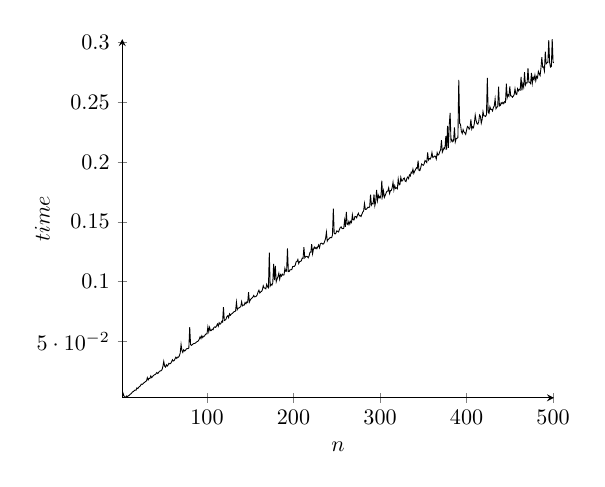
\begin{tikzpicture}[scale=0.8]
\definecolor{color0}{RGB}{0,0,0}
\begin{axis}[axis lines = middle, xmin=2.000000, xmax=501.000000,
x label style={at={(axis description cs:0.5,-0.1)},anchor=north},
y label style={at={(axis description cs:-0.15,.5)},rotate=90,anchor=south},
ymin=0.002947, ymax=0.302547, xlabel={$n$}, ylabel={$time$}]
\addplot[color0,  forget plot]
table{%
2.000000 0.002947
3.000000 0.006665
4.000000 0.004482
5.000000 0.003522
6.000000 0.003370
7.000000 0.004449
8.000000 0.003982
9.000000 0.004551
10.000000 0.004967
11.000000 0.005772
12.000000 0.006259
13.000000 0.007019
14.000000 0.007954
15.000000 0.008139
16.000000 0.009068
17.000000 0.009457
18.000000 0.009328
19.000000 0.011231
20.000000 0.010672
21.000000 0.011615
22.000000 0.012445
23.000000 0.012841
24.000000 0.014410
25.000000 0.014133
26.000000 0.014607
27.000000 0.015492
28.000000 0.015815
29.000000 0.016603
30.000000 0.016959
31.000000 0.019753
32.000000 0.017889
33.000000 0.019196
34.000000 0.019170
35.000000 0.021234
36.000000 0.019802
37.000000 0.020570
38.000000 0.021519
39.000000 0.022037
40.000000 0.022372
41.000000 0.023046
42.000000 0.024060
43.000000 0.023215
44.000000 0.024044
45.000000 0.025086
46.000000 0.025429
47.000000 0.025558
48.000000 0.026372
49.000000 0.029083
50.000000 0.033366
51.000000 0.029481
52.000000 0.028591
53.000000 0.030505
54.000000 0.029399
55.000000 0.030329
56.000000 0.031777
57.000000 0.031268
58.000000 0.031701
59.000000 0.032932
60.000000 0.034766
61.000000 0.033680
62.000000 0.033940
63.000000 0.035516
64.000000 0.036919
65.000000 0.035837
66.000000 0.036978
67.000000 0.036810
68.000000 0.037968
69.000000 0.040265
70.000000 0.047563
71.000000 0.042500
72.000000 0.040816
73.000000 0.043076
74.000000 0.042013
75.000000 0.042463
76.000000 0.043678
77.000000 0.044108
78.000000 0.043923
79.000000 0.044713
80.000000 0.062035
81.000000 0.047421
82.000000 0.046774
83.000000 0.047301
84.000000 0.048046
85.000000 0.048323
86.000000 0.048349
87.000000 0.049023
88.000000 0.049615
89.000000 0.049983
90.000000 0.050556
91.000000 0.051810
92.000000 0.053881
93.000000 0.052405
94.000000 0.054680
95.000000 0.053227
96.000000 0.054401
97.000000 0.054357
98.000000 0.055676
99.000000 0.056334
100.000000 0.056333
101.000000 0.062153
102.000000 0.058164
103.000000 0.061770
104.000000 0.058992
105.000000 0.059126
106.000000 0.060278
107.000000 0.059846
108.000000 0.061726
109.000000 0.062180
110.000000 0.061791
111.000000 0.062953
112.000000 0.064605
113.000000 0.062804
114.000000 0.065688
115.000000 0.064413
116.000000 0.064989
117.000000 0.066829
118.000000 0.066228
119.000000 0.078706
120.000000 0.067536
121.000000 0.067901
122.000000 0.068682
123.000000 0.070768
124.000000 0.071460
125.000000 0.069802
126.000000 0.073057
127.000000 0.071881
128.000000 0.072876
129.000000 0.073304
130.000000 0.073926
131.000000 0.074801
132.000000 0.075056
133.000000 0.075442
134.000000 0.082849
135.000000 0.076628
136.000000 0.077786
137.000000 0.078047
138.000000 0.078584
139.000000 0.079114
140.000000 0.083174
141.000000 0.079751
142.000000 0.080429
143.000000 0.080386
144.000000 0.082614
145.000000 0.081537
146.000000 0.083073
147.000000 0.082554
148.000000 0.091113
149.000000 0.082996
150.000000 0.084713
151.000000 0.085595
152.000000 0.086376
153.000000 0.086975
154.000000 0.088401
155.000000 0.087244
156.000000 0.087435
157.000000 0.087822
158.000000 0.089024
159.000000 0.091328
160.000000 0.092725
161.000000 0.090510
162.000000 0.091383
163.000000 0.091760
164.000000 0.093196
165.000000 0.096561
166.000000 0.094768
167.000000 0.094506
168.000000 0.093939
169.000000 0.097778
170.000000 0.095710
171.000000 0.094877
172.000000 0.124184
173.000000 0.096242
174.000000 0.097760
175.000000 0.097008
176.000000 0.098879
177.000000 0.114897
178.000000 0.101216
179.000000 0.113099
180.000000 0.099944
181.000000 0.102280
182.000000 0.104180
183.000000 0.106968
184.000000 0.102008
185.000000 0.105780
186.000000 0.104563
187.000000 0.106262
188.000000 0.105442
189.000000 0.105556
190.000000 0.111044
191.000000 0.108573
192.000000 0.108657
193.000000 0.127726
194.000000 0.108369
195.000000 0.108457
196.000000 0.109960
197.000000 0.109921
198.000000 0.110025
199.000000 0.112547
200.000000 0.112708
201.000000 0.112732
202.000000 0.113704
203.000000 0.116536
204.000000 0.116791
205.000000 0.118458
206.000000 0.115104
207.000000 0.116650
208.000000 0.116932
209.000000 0.117314
210.000000 0.119533
211.000000 0.119386
212.000000 0.128694
213.000000 0.119844
214.000000 0.120803
215.000000 0.121055
216.000000 0.120866
217.000000 0.119904
218.000000 0.121551
219.000000 0.124414
220.000000 0.124529
221.000000 0.131359
222.000000 0.123313
223.000000 0.126977
224.000000 0.128872
225.000000 0.127579
226.000000 0.128597
227.000000 0.127477
228.000000 0.129040
229.000000 0.130606
230.000000 0.128261
231.000000 0.131442
232.000000 0.132114
233.000000 0.131908
234.000000 0.131216
235.000000 0.131715
236.000000 0.133783
237.000000 0.135859
238.000000 0.141234
239.000000 0.133858
240.000000 0.135174
241.000000 0.135689
242.000000 0.136672
243.000000 0.136814
244.000000 0.136688
245.000000 0.138898
246.000000 0.161005
247.000000 0.140342
248.000000 0.139803
249.000000 0.140438
250.000000 0.142391
251.000000 0.141978
252.000000 0.141481
253.000000 0.143451
254.000000 0.145196
255.000000 0.145712
256.000000 0.144448
257.000000 0.144229
258.000000 0.144410
259.000000 0.151152
260.000000 0.145678
261.000000 0.158151
262.000000 0.148179
263.000000 0.147456
264.000000 0.150274
265.000000 0.148058
266.000000 0.150395
267.000000 0.149385
268.000000 0.155776
269.000000 0.151506
270.000000 0.151474
271.000000 0.154442
272.000000 0.154321
273.000000 0.153329
274.000000 0.155776
275.000000 0.157105
276.000000 0.154912
277.000000 0.155094
278.000000 0.154315
279.000000 0.156210
280.000000 0.158039
281.000000 0.158986
282.000000 0.165292
283.000000 0.160313
284.000000 0.160354
285.000000 0.161092
286.000000 0.162191
287.000000 0.161834
288.000000 0.162504
289.000000 0.172613
290.000000 0.163959
291.000000 0.165451
292.000000 0.165040
293.000000 0.172866
294.000000 0.163451
295.000000 0.166907
296.000000 0.176541
297.000000 0.167855
298.000000 0.172165
299.000000 0.169955
300.000000 0.171213
301.000000 0.169863
302.000000 0.184292
303.000000 0.171537
304.000000 0.175816
305.000000 0.170380
306.000000 0.172070
307.000000 0.174044
308.000000 0.175466
309.000000 0.175558
310.000000 0.178396
311.000000 0.173603
312.000000 0.176000
313.000000 0.176143
314.000000 0.178423
315.000000 0.182975
316.000000 0.176581
317.000000 0.180145
318.000000 0.177789
319.000000 0.178441
320.000000 0.177589
321.000000 0.185601
322.000000 0.180799
323.000000 0.181025
324.000000 0.187094
325.000000 0.183961
326.000000 0.184191
327.000000 0.186017
328.000000 0.186566
329.000000 0.184039
330.000000 0.183538
331.000000 0.186288
332.000000 0.187330
333.000000 0.186067
334.000000 0.189161
335.000000 0.188296
336.000000 0.191473
337.000000 0.190678
338.000000 0.193956
339.000000 0.190386
340.000000 0.192280
341.000000 0.193498
342.000000 0.195111
343.000000 0.194482
344.000000 0.201023
345.000000 0.192794
346.000000 0.192630
347.000000 0.195096
348.000000 0.198217
349.000000 0.197629
350.000000 0.197143
351.000000 0.198412
352.000000 0.201212
353.000000 0.200470
354.000000 0.199481
355.000000 0.207967
356.000000 0.201650
357.000000 0.202835
358.000000 0.202349
359.000000 0.203915
360.000000 0.207761
361.000000 0.203695
362.000000 0.204102
363.000000 0.204871
364.000000 0.204634
365.000000 0.202455
366.000000 0.207660
367.000000 0.205666
368.000000 0.206203
369.000000 0.208534
370.000000 0.210104
371.000000 0.218138
372.000000 0.208163
373.000000 0.209919
374.000000 0.211862
375.000000 0.210935
376.000000 0.221426
377.000000 0.210254
378.000000 0.230017
379.000000 0.211816
380.000000 0.231004
381.000000 0.240988
382.000000 0.217111
383.000000 0.218613
384.000000 0.216856
385.000000 0.217687
386.000000 0.228795
387.000000 0.216719
388.000000 0.219408
389.000000 0.219768
390.000000 0.220251
391.000000 0.268573
392.000000 0.232185
393.000000 0.231328
394.000000 0.225510
395.000000 0.223789
396.000000 0.226949
397.000000 0.225042
398.000000 0.224299
399.000000 0.223017
400.000000 0.226498
401.000000 0.229677
402.000000 0.229017
403.000000 0.227371
404.000000 0.228461
405.000000 0.235532
406.000000 0.227508
407.000000 0.229407
408.000000 0.228540
409.000000 0.232207
410.000000 0.239123
411.000000 0.234561
412.000000 0.232104
413.000000 0.231506
414.000000 0.233372
415.000000 0.239189
416.000000 0.238212
417.000000 0.232387
418.000000 0.235463
419.000000 0.241987
420.000000 0.238442
421.000000 0.238475
422.000000 0.237934
423.000000 0.239457
424.000000 0.270117
425.000000 0.241312
426.000000 0.240534
427.000000 0.245966
428.000000 0.243850
429.000000 0.243931
430.000000 0.242583
431.000000 0.245443
432.000000 0.246627
433.000000 0.252679
434.000000 0.244419
435.000000 0.245698
436.000000 0.246077
437.000000 0.262874
438.000000 0.246679
439.000000 0.247038
440.000000 0.249432
441.000000 0.248638
442.000000 0.249758
443.000000 0.248662
444.000000 0.250331
445.000000 0.249767
446.000000 0.265268
447.000000 0.253695
448.000000 0.256053
449.000000 0.254894
450.000000 0.262962
451.000000 0.255181
452.000000 0.255060
453.000000 0.254005
454.000000 0.254875
455.000000 0.256180
456.000000 0.261072
457.000000 0.256722
458.000000 0.256297
459.000000 0.261084
460.000000 0.259366
461.000000 0.260720
462.000000 0.260086
463.000000 0.271060
464.000000 0.259872
465.000000 0.265239
466.000000 0.262336
467.000000 0.274933
468.000000 0.264229
469.000000 0.266044
470.000000 0.265923
471.000000 0.278316
472.000000 0.266599
473.000000 0.266443
474.000000 0.265408
475.000000 0.274268
476.000000 0.265675
477.000000 0.270702
478.000000 0.268846
479.000000 0.272576
480.000000 0.267817
481.000000 0.271384
482.000000 0.270198
483.000000 0.275586
484.000000 0.273648
485.000000 0.272081
486.000000 0.278432
487.000000 0.287419
488.000000 0.279054
489.000000 0.279265
490.000000 0.276041
491.000000 0.292127
492.000000 0.281955
493.000000 0.282787
494.000000 0.283163
495.000000 0.301702
496.000000 0.283105
497.000000 0.279156
498.000000 0.279792
499.000000 0.302547
500.000000 0.283238
501.000000 0.282748
};
\end{axis}
\end{tikzpicture}

   \end{center}
   \captionof{figure}{\label{fig:time}Plot of the time in seconds required to
   compute the approximation for $n\in(2,502)$.}
\end{Figure}

This can be somewhat decreased through parallel processing, as the computation
of the local system of equations is independent. Thus this process can be
split into multiple processes. However, due to the efficiency of this system on
one dimension, this will only reduce the complexity to $\approx O(2N)$.

\begin{Figure}
   \begin{center}
     \begin{tikzpicture}
\definecolor{color0}{RGB}{0,0,0}
\definecolor{color1}{RGB}{0,0,0}
\begin{axis}[axis lines = middle, xmin=0.000000, xmax=4.975000, ymin=-1.000000, ymax=1.000000]
\addplot[color0, dashed,  forget plot]
table{%
0.000000 0.000000
0.025000 0.031411
0.050000 0.062791
0.075000 0.094108
0.100000 0.125333
0.125000 0.156434
0.150000 0.187381
0.175000 0.218143
0.200000 0.248690
0.225000 0.278991
0.250000 0.309017
0.275000 0.338738
0.300000 0.368125
0.325000 0.397148
0.350000 0.425779
0.375000 0.453990
0.400000 0.481754
0.425000 0.509041
0.450000 0.535827
0.475000 0.562083
0.500000 0.587785
0.525000 0.612907
0.550000 0.637424
0.575000 0.661312
0.600000 0.684547
0.625000 0.707107
0.650000 0.728969
0.675000 0.750111
0.700000 0.770513
0.725000 0.790155
0.750000 0.809017
0.775000 0.827081
0.800000 0.844328
0.825000 0.860742
0.850000 0.876307
0.875000 0.891007
0.900000 0.904827
0.925000 0.917755
0.950000 0.929776
0.975000 0.940881
1.000000 0.951057
1.025000 0.960294
1.050000 0.968583
1.075000 0.975917
1.100000 0.982287
1.125000 0.987688
1.150000 0.992115
1.175000 0.995562
1.200000 0.998027
1.225000 0.999507
1.250000 1.000000
1.275000 0.999507
1.300000 0.998027
1.325000 0.995562
1.350000 0.992115
1.375000 0.987688
1.400000 0.982287
1.425000 0.975917
1.450000 0.968583
1.475000 0.960294
1.500000 0.951057
1.525000 0.940881
1.550000 0.929776
1.575000 0.917755
1.600000 0.904827
1.625000 0.891007
1.650000 0.876307
1.675000 0.860742
1.700000 0.844328
1.725000 0.827081
1.750000 0.809017
1.775000 0.790155
1.800000 0.770513
1.825000 0.750111
1.850000 0.728969
1.875000 0.707107
1.900000 0.684547
1.925000 0.661312
1.950000 0.637424
1.975000 0.612907
2.000000 0.587785
2.025000 0.562083
2.050000 0.535827
2.075000 0.509041
2.100000 0.481754
2.125000 0.453990
2.150000 0.425779
2.175000 0.397148
2.200000 0.368125
2.225000 0.338738
2.250000 0.309017
2.275000 0.278991
2.300000 0.248690
2.325000 0.218143
2.350000 0.187381
2.375000 0.156434
2.400000 0.125333
2.425000 0.094108
2.450000 0.062791
2.475000 0.031411
2.500000 0.000000
2.525000 -0.031411
2.550000 -0.062791
2.575000 -0.094108
2.600000 -0.125333
2.625000 -0.156434
2.650000 -0.187381
2.675000 -0.218143
2.700000 -0.248690
2.725000 -0.278991
2.750000 -0.309017
2.775000 -0.338738
2.800000 -0.368125
2.825000 -0.397148
2.850000 -0.425779
2.875000 -0.453990
2.900000 -0.481754
2.925000 -0.509041
2.950000 -0.535827
2.975000 -0.562083
3.000000 -0.587785
3.025000 -0.612907
3.050000 -0.637424
3.075000 -0.661312
3.100000 -0.684547
3.125000 -0.707107
3.150000 -0.728969
3.175000 -0.750111
3.200000 -0.770513
3.225000 -0.790155
3.250000 -0.809017
3.275000 -0.827081
3.300000 -0.844328
3.325000 -0.860742
3.350000 -0.876307
3.375000 -0.891007
3.400000 -0.904827
3.425000 -0.917755
3.450000 -0.929776
3.475000 -0.940881
3.500000 -0.951057
3.525000 -0.960294
3.550000 -0.968583
3.575000 -0.975917
3.600000 -0.982287
3.625000 -0.987688
3.650000 -0.992115
3.675000 -0.995562
3.700000 -0.998027
3.725000 -0.999507
3.750000 -1.000000
3.775000 -0.999507
3.800000 -0.998027
3.825000 -0.995562
3.850000 -0.992115
3.875000 -0.987688
3.900000 -0.982287
3.925000 -0.975917
3.950000 -0.968583
3.975000 -0.960294
4.000000 -0.951057
4.025000 -0.940881
4.050000 -0.929776
4.075000 -0.917755
4.100000 -0.904827
4.125000 -0.891007
4.150000 -0.876307
4.175000 -0.860742
4.200000 -0.844328
4.225000 -0.827081
4.250000 -0.809017
4.275000 -0.790155
4.300000 -0.770513
4.325000 -0.750111
4.350000 -0.728969
4.375000 -0.707107
4.400000 -0.684547
4.425000 -0.661312
4.450000 -0.637424
4.475000 -0.612907
4.500000 -0.587785
4.525000 -0.562083
4.550000 -0.535827
4.575000 -0.509041
4.600000 -0.481754
4.625000 -0.453990
4.650000 -0.425779
4.675000 -0.397148
4.700000 -0.368125
4.725000 -0.338738
4.750000 -0.309017
4.775000 -0.278991
4.800000 -0.248690
4.825000 -0.218143
4.850000 -0.187381
4.875000 -0.156434
4.900000 -0.125333
4.925000 -0.094108
4.950000 -0.062791
4.975000 -0.031411
};
\addplot[color1,  forget plot]
table{%
0.000000 0.000000
0.025000 0.031410
0.050000 0.062791
0.075000 0.094107
0.100000 0.125334
0.125000 0.156432
0.150000 0.187382
0.175000 0.218140
0.200000 0.248690
0.225000 0.278987
0.250000 0.309017
0.275000 0.338733
0.300000 0.368124
0.325000 0.397142
0.350000 0.425779
0.375000 0.453983
0.400000 0.481753
0.425000 0.509033
0.450000 0.535825
0.475000 0.562074
0.500000 0.587783
0.525000 0.612897
0.550000 0.637421
0.575000 0.661301
0.600000 0.684543
0.625000 0.707095
0.650000 0.728964
0.675000 0.750099
0.700000 0.770508
0.725000 0.790142
0.750000 0.809010
0.775000 0.827067
0.800000 0.844320
0.825000 0.860728
0.850000 0.876298
0.875000 0.890992
0.900000 0.904817
0.925000 0.917740
0.950000 0.929766
0.975000 0.940866
1.000000 0.951045
1.025000 0.960278
1.050000 0.968571
1.075000 0.975901
1.100000 0.982274
1.125000 0.987672
1.150000 0.992100
1.175000 0.995546
1.200000 0.998011
1.225000 0.999490
1.250000 0.999984
1.275000 0.999490
1.300000 0.998010
1.325000 0.995546
1.350000 0.992097
1.375000 0.987672
1.400000 0.982269
1.425000 0.975901
1.450000 0.968564
1.475000 0.960278
1.500000 0.951037
1.525000 0.940865
1.550000 0.929757
1.575000 0.917739
1.600000 0.904807
1.625000 0.890992
1.650000 0.876286
1.675000 0.860727
1.700000 0.844307
1.725000 0.827066
1.750000 0.808996
1.775000 0.790141
1.800000 0.770493
1.825000 0.750097
1.850000 0.728948
1.875000 0.707093
1.900000 0.684527
1.925000 0.661299
1.950000 0.637404
1.975000 0.612894
2.000000 0.587765
2.025000 0.562071
2.050000 0.535807
2.075000 0.509029
2.100000 0.481735
2.125000 0.453978
2.150000 0.425761
2.175000 0.397136
2.200000 0.368107
2.225000 0.338726
2.250000 0.309000
2.275000 0.278979
2.300000 0.248674
2.325000 0.218131
2.350000 0.187366
2.375000 0.156422
2.400000 0.125319
2.425000 0.094096
2.450000 0.062777
2.475000 0.031398
2.500000 -0.000013
2.525000 -0.031424
2.550000 -0.062802
2.575000 -0.094122
2.600000 -0.125344
2.625000 -0.156448
2.650000 -0.187391
2.675000 -0.218157
2.700000 -0.248699
2.725000 -0.279004
2.750000 -0.309025
2.775000 -0.338751
2.800000 -0.368132
2.825000 -0.397160
2.850000 -0.425785
2.875000 -0.454003
2.900000 -0.481759
2.925000 -0.509053
2.950000 -0.535831
2.975000 -0.562094
3.000000 -0.587789
3.025000 -0.612917
3.050000 -0.637427
3.075000 -0.661321
3.100000 -0.684549
3.125000 -0.707115
3.150000 -0.728970
3.175000 -0.750119
3.200000 -0.770514
3.225000 -0.790162
3.250000 -0.809017
3.275000 -0.827086
3.300000 -0.844327
3.325000 -0.860747
3.350000 -0.876305
3.375000 -0.891010
3.400000 -0.904825
3.425000 -0.917757
3.450000 -0.929774
3.475000 -0.940883
3.500000 -0.951054
3.525000 -0.960294
3.550000 -0.968580
3.575000 -0.975917
3.600000 -0.982284
3.625000 -0.987687
3.650000 -0.992112
3.675000 -0.995560
3.700000 -0.998023
3.725000 -0.999504
3.750000 -0.999997
3.775000 -0.999503
3.800000 -0.998023
3.825000 -0.995558
3.850000 -0.992111
3.875000 -0.987683
3.900000 -0.982284
3.925000 -0.975911
3.950000 -0.968580
3.975000 -0.960287
4.000000 -0.951054
4.025000 -0.940874
4.050000 -0.929774
4.075000 -0.917747
4.100000 -0.904825
4.125000 -0.890999
4.150000 -0.876305
4.175000 -0.860734
4.200000 -0.844326
4.225000 -0.827073
4.250000 -0.809016
4.275000 -0.790147
4.300000 -0.770512
4.325000 -0.750103
4.350000 -0.728968
4.375000 -0.707099
4.400000 -0.684547
4.425000 -0.661304
4.450000 -0.637424
4.475000 -0.612900
4.500000 -0.587785
4.525000 -0.562077
4.550000 -0.535827
4.575000 -0.509035
4.600000 -0.481754
4.625000 -0.453985
4.650000 -0.425780
4.675000 -0.397143
4.700000 -0.368125
4.725000 -0.338733
4.750000 -0.309018
4.775000 -0.278987
4.800000 -0.248691
4.825000 -0.218140
4.850000 -0.187382
4.875000 -0.156432
4.900000 -0.125334
4.925000 -0.094107
4.950000 -0.062791
4.975000 -0.031410
};
\end{axis}
\end{tikzpicture}

   \end{center}
  \captionof{figure}{$T_h(x)$ compared to $\sin\left(\frac{2\pi}{5}x\right)$,
  when $N=500$.}
  \label{fig:example_500}
\end{Figure}

Figure \ref{fig:example_500} demonstrates the accuracy of the approximation for
very large $N$ values. In this case with $N=500$ the error can be neglected, as
it is on the order of $10^{-5}$. This simple demonstration shows the strength
of FEA, and how it can be applied to a simple one dimensional differential
equation.

\section{Conclusion}%
\label{sec:conclusion}

The method of finite element analysis constrained in one dimension is not
extensively useful, as the analytic solutions for most differential equations is
possible to compute without much difficulty. However, this demonstration and
explanation of FEA shows the ability of of the process in comparison to an
actual solution. And provides a generalizable process that can be expanded to
higher dimensional problems.

As it was noted in the example problem, much of this process can be automated.
The only parts that require manual work are the theoretical stages, and after
than all other stages of the approximation process can be automated by a
computer. This allows for much simpler process, as human work is only necessary
for a change of dimension or a change of differential equation. All other
altercations to the initial conditions, or the forcing function can be handled
by computers.

\end{multicols}

\newpage

\nocite{*}
\bibliographystyle{alpha}
\bibliography{fem}

\end{document}
